%\documentclass{beamer}
\documentclass[a4paper]{article}
% \documentclass[10pt]{article}

\usepackage{float}
\usepackage{ctex}
\usepackage{graphicx} 
\usepackage{geometry}
\usepackage{tikz}
\usepackage{amsmath}
\usepackage{setspace}
\usepackage{subcaption}
% for table
\usepackage{tabularx}

%引入python/matlab包
\usepackage{listings}
\usepackage{color}
\definecolor{dkgreen}{rgb}{0,0.6,0}
\definecolor{gray}{rgb}{0.5,0.5,0.5}
\definecolor{mauve}{rgb}{0.58,0,0.82}
\lstset{frame=tb,
  language=Python,
  aboveskip=3mm,
  belowskip=3mm,
  showstringspaces=false,
  columns=flexible,
  basicstyle={\small\ttfamily},
  numbers=left,%设置行号位置none不显示行号
  %numberstyle=\tiny\courier, %设置行号大小
  numberstyle=\tiny\color{gray},
  keywordstyle=\color{blue},
  commentstyle=\color{dkgreen},
  stringstyle=\color{mauve},
  breaklines=true,
  breakatwhitespace=true,
  escapeinside=``,%逃逸字符(1左面的键),用于显示中文例如在代码中`中文...`
  tabsize=4,
  extendedchars=false %解决代码跨页时,章节标题,页眉等汉字不显示的问题
}


\definecolor{mygreen}{rgb}{0,0.6,0}
\definecolor{mygray}{rgb}{0.5,0.5,0.5}
\definecolor{mymauve}{rgb}{0.58,0,0.82}



\usetikzlibrary{positioning, shapes.geometric}
%\usepackage[english, chinese]{babel}

% \usepackage{polyglossia}
% \setmainlanguage{english}
% \setotherlanguage{chinese}
%设置段间距
\setlength{\parskip}{1em}
%设置行间距
\renewcommand{\baselinestretch}{1.5}


\geometry{left=2.54cm, right=2.54cm, top=3.18cm, bottom=3.18cm}
\graphicspath{{./figures/}}
%\newcommand{\myud}{\textbf{}}

\title{Unified Vision-Language Pre-Training for Image Captioning and VQA}
\author{LoongCat}
\date{\today}
\begin{document}
\begin{sloppypar}
    \maketitle
    \section{Structure}


    \begin{figure}[H]
        \centering
        \begin{minipage}{0.49\linewidth}
            \centering
            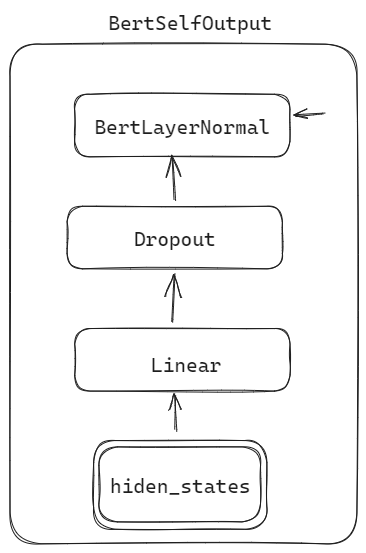
\includegraphics[width=3.15in,height=3.0in]{BertOutput}
            \caption{BertSelfOutput}
            \label{BertSelfOutput}%文中引用该图片代号
        \end{minipage}
        %\qquad
        \begin{minipage}{0.49\linewidth}
            \centering
            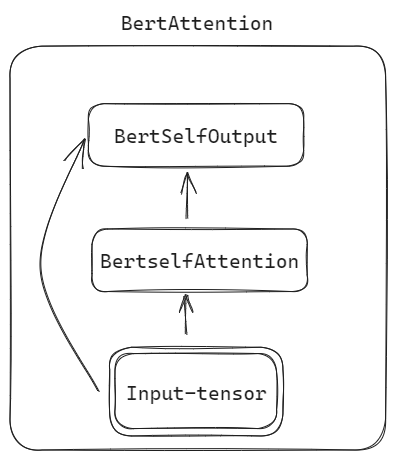
\includegraphics[width=3.15in,height=3.0in]{BertAttention}
            \caption{BertAttention}
            \label{BertAttention}%文中引用该图片代号
        \end{minipage}

    \end{figure}

    \begin{figure}[H]
        \centering
        \begin{minipage}{0.49\linewidth}
            \centering
            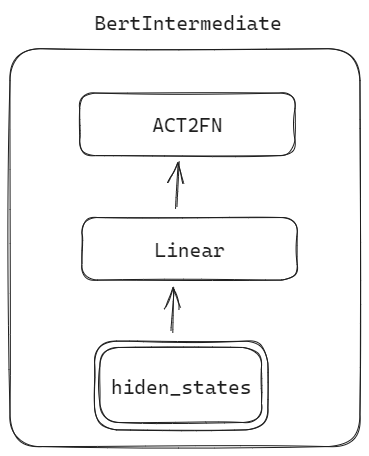
\includegraphics[width=3.15in,height=3.0in]{BertIntermediate}
            \caption{BertIntermediate}
            \label{BertIntermediate}%文中引用该图片代号
        \end{minipage}
        %\qquad
        \begin{minipage}{0.49\linewidth}
            \centering
            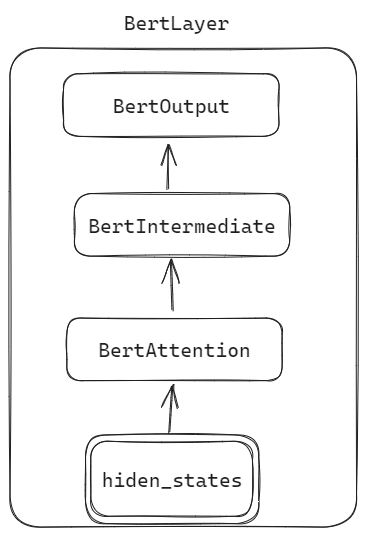
\includegraphics[width=3.15in,height=3.0in]{BertLayer}
            \caption{BertLayer}
            \label{BertLayer}%文中引用该图片代号
        \end{minipage}

    \end{figure}


    BertConfig类代码:关注:num\_hidden\_layers=12,有12个Layer

    \begin{lstlisting}
          class BertConfig(object):
                """Configuration class to store the configuration of a `BertModel`.
                """
          
                def __init__(self,
                            vocab_size_or_config_json_file,
                            hidden_size=768,
                            num_hidden_layers=12,
                            num_attention_heads=12,
                            intermediate_size=3072,
                            hidden_act="gelu",
                            hidden_dropout_prob=0.1,
                            attention_probs_dropout_prob=0.1,
                            max_position_embeddings=512,
                            type_vocab_size=2,
                            relax_projection=0,
                            initializer_range=0.02,
                            task_idx=None,
                            fp32_embedding=False,
                            label_smoothing=None):
    \end{lstlisting}

    BertEncoder类代码:关注:self.layer

    \begin{lstlisting}
          class BertEncoder(nn.Module):
                def __init__(self, config):
                    super(BertEncoder, self).__init__()
                    layer = BertLayer(config)
                    self.layer = nn.ModuleList([copy.deepcopy(layer)
                                                for _ in range(config.num_hidden_layers)])
          
                def forward(self, hidden_states, attention_mask, prev_embedding=None, prev_encoded_layers=None, output_all_encoded_layers=True):
                    assert (prev_embedding is None) == (prev_encoded_layers is None), \
                                "history embedding and encoded layer must be simultanously given."
                    all_encoder_layers = []
                    if (prev_embedding is not None) and (prev_encoded_layers is not None):
                        history_states = prev_embedding
                        for i, layer_module in enumerate(self.layer):
                                hidden_states = layer_module(
                                hidden_states, attention_mask, history_states=history_states)
                                if output_all_encoded_layers:
                                all_encoder_layers.append(hidden_states)
                                if prev_encoded_layers is not None:
                                history_states = prev_encoded_layers[i]
                    else:
                        for layer_module in self.layer:
                                hidden_states = layer_module(hidden_states, attention_mask)
                                if output_all_encoded_layers:
                                all_encoder_layers.append(hidden_states)
                    if not output_all_encoded_layers:
                        all_encoder_layers.append(hidden_states)
                    return all_encoder_layers
          \end{lstlisting}

    $hidden\_states = layer\_module(hidden\_states, attention\_mask)$ 这行就是表明:
    $$
        H_l = Transformer(H_{l - 1}),l \in [1,L]
    $$


    \begin{figure}[H]
        \centering
        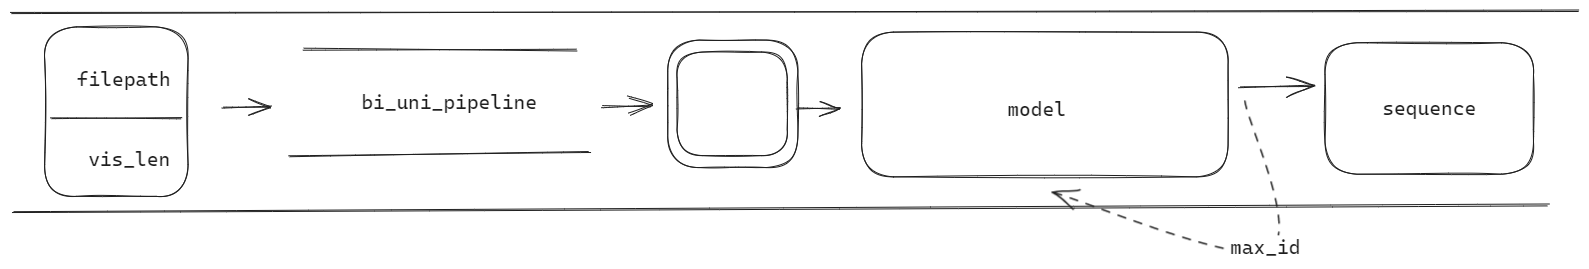
\includegraphics[scale=0.5]{ProcDecoder.png}

        %\caption{Bert4S2SDecoder,生成过程由next_pos < output_length:该语句控制,没体现出来STOP标记的作用}
        \caption{decode\_img2txt文件中提供了i2t的方法,首先建立一个preprocess管道bi\_uni\_pipeline(来自于s2s\_loader的Preprocess4Seq2seqDecoder)
            用来预处理输入的图像
            管道的输入:图像路径与图像大小
            管道的输出:input\_id,..position\_ids,..input\_mask等
            管道的输出用instances来接收,再次经过处理之后,输送给model模型,为modeling的BertForSeq2SeqDecoder类对象,
            model输入:vis\_feat,vis\_pe,..attention\_mask等
            model输出:max\_ids,max\_probs
        }

        \label{ProcDecoder}
        %\caption{整个过程是由\textbf{while next_pos < output_length}控制的,没体现出来到\textbf{STOP}标记停止生成}
    \end{figure}


    \begin{figure}[H]
        \centering
        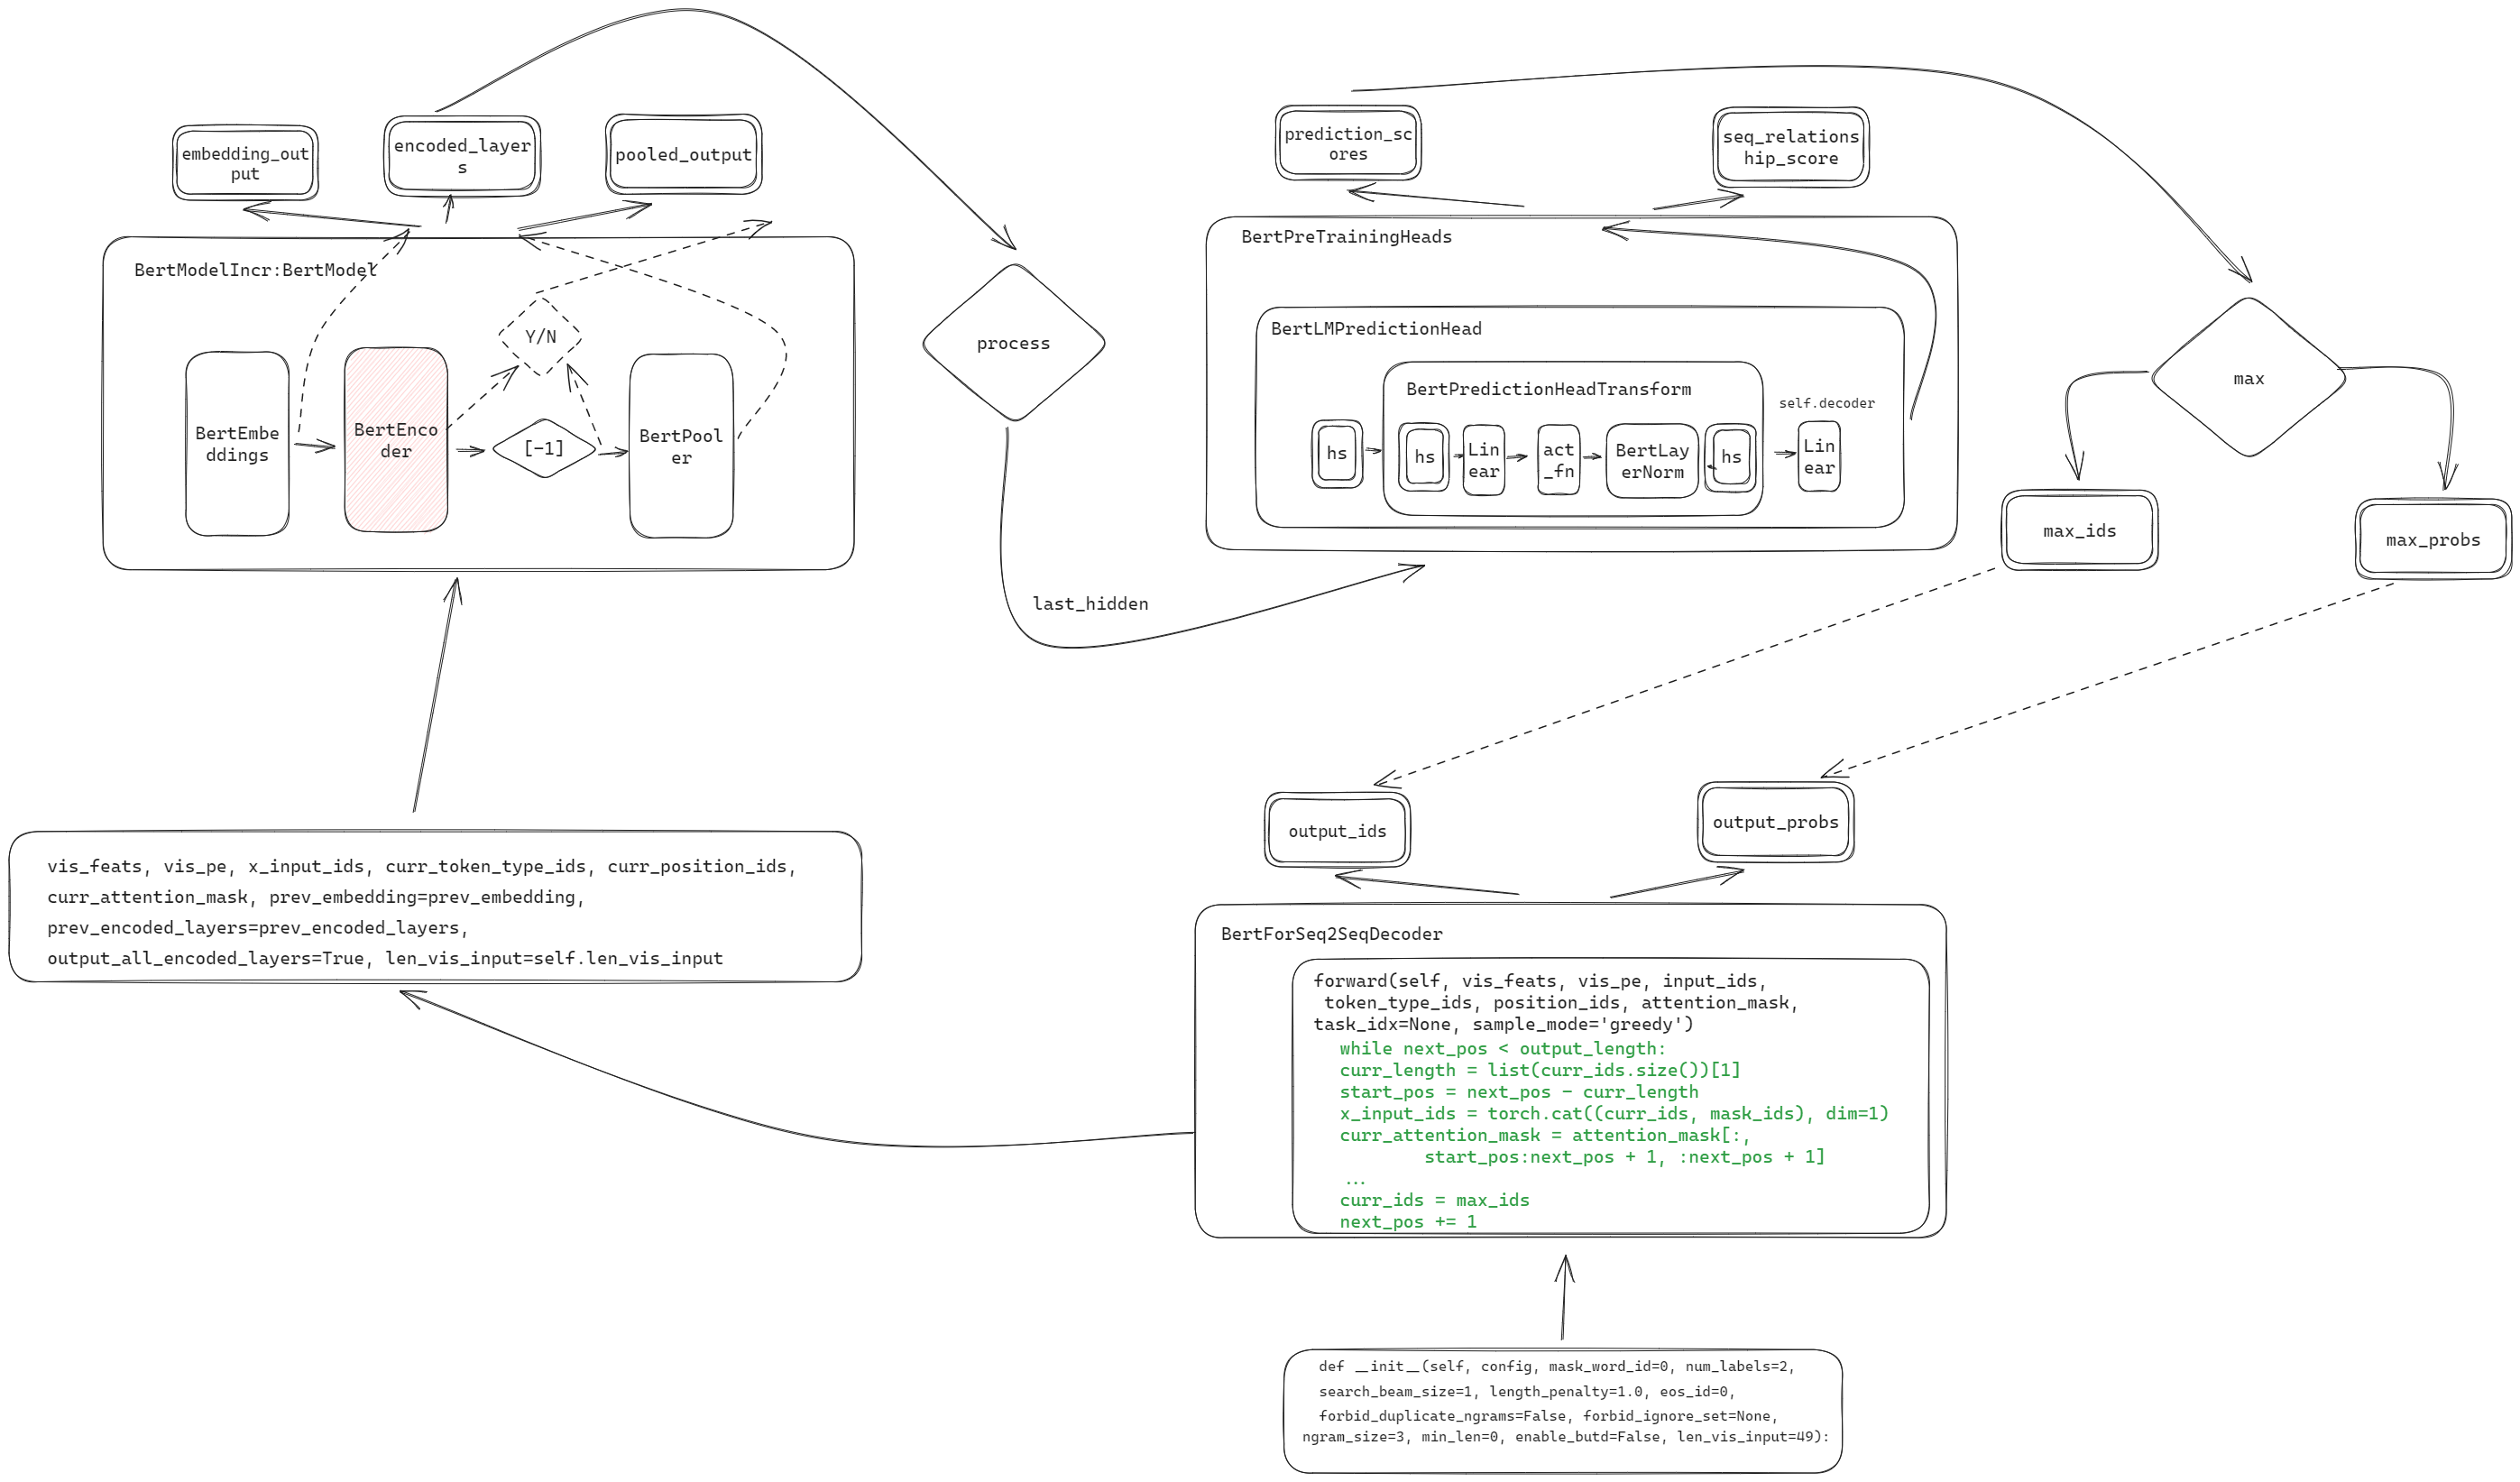
\includegraphics[width=6.5in,height=5.0in]{Bert4S2SDecoder.png}

        %\caption{Bert4S2SDecoder,生成过程由next_pos < output_length:该语句控制,没体现出来STOP标记的作用}
        \caption{Bert4S2SDecoder, 生成过程由 next\_pos \textless output\_length: 该语句控制,没体现出来 STOP 标记的作用}

        \label{Bert4S2SDecoder}
        %\caption{整个过程是由\textbf{while next_pos < output_length}控制的,没体现出来到\textbf{STOP}标记停止生成}
    \end{figure}


    \newpage
    decoder\_img2txt.py:
    \begin{lstlisting}
          #一个预处理图像的管道
          #输入图像路径和图像大小
          #返回input_ids, segment_ids(token_type_ids), position_ids, input_mask, task_idx, img, vis_pe
          bi_uni_pipeline = []
          bi_uni_pipeline.append(seq2seq_loader.Preprocess4Seq2seqDecoder(list(
              tokenizer.vocab.keys()), tokenizer.convert_tokens_to_ids, args.max_seq_length,
              max_tgt_length=args.max_tgt_length, new_segment_ids=args.new_segment_ids,
              mode='s2s', len_vis_input=args.len_vis_input, enable_butd=args.enable_butd,
              region_bbox_file=args.region_bbox_file, region_det_file_prefix=args.region_det_file_prefix))
          ...

          #用来解码的模型
          #输入时
          model = BertForSeq2SeqDecoder.from_pretrained(args.bert_model,
                max_position_embeddings=args.max_position_embeddings, config_path=args.config_path,
                state_dict=model_recover, num_labels=cls_num_labels,
                type_vocab_size=type_vocab_size, task_idx=3, mask_word_id=mask_word_id,
                search_beam_size=args.beam_size, length_penalty=args.length_penalty,
                eos_id=eos_word_ids, forbid_duplicate_ngrams=args.forbid_duplicate_ngrams,
                forbid_ignore_set=forbid_ignore_set, ngram_size=args.ngram_size, min_len=args.min_len,
                enable_butd=args.enable_butd, len_vis_input=args.len_vis_input)

          ...

          for src in img_dat:
                src_tk = os.path.join(args.image_root, src.get('filepath', 'trainval'), src['filename'])
                input_lines.append((img_idx, imgid, src_tk))


          ...

          _chunk = input_lines[next_i:next_i + args.batch_size]
          buf = [x[2] for x in _chunk]
          # instance 其实就是图像路径和输入图像大小的一个元组
          for instance in [(x, args.len_vis_input) for x in buf]:
            #用 instances 来接收图像预处理的输出
            for proc in bi_uni_pipeline:
                instances.append(proc(instance))

          ...

          input_ids, token_type_ids, position_ids, input_mask, task_idx, img, vis_pe = batch

          #将管道的输出处理之后送入解码模型
          #输出 max_id 与 max_prob
          traces = model(conv_feats, vis_pe, input_ids, token_type_ids,
                                 position_ids, input_mask, task_idx=task_idx)
          
          #将返回的 max_id 转换为 tokens
          output_buf = tokenizer.convert_ids_to_tokens(w_ids)
          output_tokens = []
          #将非标记 tokens 提取出来
          for t in output_buf:
                if t in ("[SEP]", "[PAD]"):
                      break
                output_tokens.append(t)
          # tokens 变句子?
          output_sequence = ' '.join(detokenize(output_tokens))
          #记录每个图片id对应的句子描述
          output_lines[buf_id[i]] = output_sequence
          #图像标记序号为 tup[1] 的描述为 output_lines[imd_idx]
          predictions = [{'image_id': tup[1], 'caption': output_lines[img_idx]} for img_idx, tup in enumerate(input_lines)]
          \end{lstlisting}



    \newpage

    seq2seq\_loader.py:
    \begin{lstlisting}
          #全1 的下三角矩阵,创建 MASKED 矩阵用
          self._tril_matrix = torch.tril(torch.ones(
                (max_len, max_len), dtype=torch.long))

          
          def __call__(self, instance):
            img_path, max_a_len = instance[:2]
            tokens_a = ['[UNK]'] * self.len_vis_input
        
            # Add Special Tokens
            padded_tokens_a = ['[CLS]'] + tokens_a + ['[SEP]']
            tokens = padded_tokens_a
            if self.new_segment_ids:
                segment_ids = [4]*(len(padded_tokens_a)) \
                    + [5]*(max_len_in_batch - len(padded_tokens_a))
            else:
                segment_ids = [0]*(len(padded_tokens_a)) \
                    + [1]*(max_len_in_batch - len(padded_tokens_a))
            ...

            position_ids = []
            for i in range(len(tokens_a) + 2):
                    position_ids.append(i)
            for i in range(len(tokens_a) + 2, max_a_len + 2):
                    position_ids.append(0)
            for i in range(max_a_len + 2, max_len_in_batch):
                    position_ids.append(i - (max_a_len + 2) + len(tokens_a) + 2)
        
            # Token Indexing
            input_ids = self.indexer(tokens)
        
            # Zero Padding
            #首先创建一个全 0 的矩阵
            input_mask = torch.zeros(
                    max_len_in_batch, max_len_in_batch, dtype=torch.long)
            #图像区域填充 1
            input_mask[:, :len(tokens_a)+2].fill_(1)

            second_st, second_end = len(padded_tokens_a), max_len_in_batch
        
            #句子部分拷贝全 1 矩阵的句子部分 tokens 长度的下三角矩阵
            input_mask[second_st:second_end, second_st:second_end].copy_(
                    self._tril_matrix[:second_end-second_st, :second_end-second_st])
        
            img = torch.from_numpy(region_feat_f[img_id][:]).float()
            vis_pe = torch.from_numpy(region_bbox_f[img_id][:])

            # lazy normalization of the coordinates...
            w_est = torch.max(vis_pe[:, [0, 2]])*1.+1e-5
            h_est = torch.max(vis_pe[:, [1, 3]])*1.+1e-5
            vis_pe[:, [0, 2]] /= w_est
            vis_pe[:, [1, 3]] /= h_est
            rel_area = (vis_pe[:, 3]-vis_pe[:, 1])*(vis_pe[:, 2]-vis_pe[:, 0])
            rel_area.clamp_(0)
            vis_pe = torch.cat((vis_pe[:, :4], rel_area.view(-1, 1), vis_pe[:, 5:]), -1) # confident score
            normalized_coord = F.normalize(vis_pe.data[:, :5]-0.5, dim=-1)
            vis_pe = torch.cat((F.layer_norm(vis_pe, [6]), \
                    F.layer_norm(cls_label, [1601])), dim=-1) # 1601 hard coded...

            return (input_ids, segment_ids, position_ids, input_mask, self.task_idx, img, vis_pe)
    \end{lstlisting}

    \newpage

    modeling.py:BertForSeq2SeqDecoder
    \begin{lstlisting}
        #输出隐藏层的解码器,输入为:图像特征 , word_id , attention_mask , 参数矩阵等
        self.bert = BertModelIncr(config)
        #输出预测结果的解码器,输入为隐藏层状态
        self.cls = BertPreTrainingHeads(
            config, self.bert.embeddings.word_embeddings.weight, num_labels=num_labels)


        def forward(self, vis_feats, vis_pe, input_ids, token_type_ids, position_ids, attention_mask, task_idx=None, sample_mode='greedy'):

            vis_feats = self.vis_embed(vis_feats) # image region features
            vis_pe = self.vis_pe_embed(vis_pe) # image region positional encodings

            ...
            mask_ids = input_ids[:, :1] * 0 + self.mask_word_id
            next_pos =  list(input_ids.size())[1]
            output_length = list(token_type_ids.size())[1]

            while next_pos < output_length:
                curr_length = list(curr_ids.size())[1]
                start_pos = next_pos - curr_length
                #把当前的输出当做输入来产生下一个词
                x_input_ids = torch.cat((curr_ids, mask_ids), dim=1)
                curr_token_type_ids = token_type_ids[:, start_pos:next_pos + 1]
                #实时更新传入的 MASKED 矩阵
                curr_attention_mask = attention_mask[:,
                    start_pos:next_pos + 1, :next_pos + 1]
                #更新pos矩阵
                curr_position_ids = position_ids[:, start_pos:next_pos + 1]
                #将图像与当前产生的 token 送入 decoer 模块,产生所有 hidden_states 层的输出
                new_embedding, new_encoded_layers, _ = \
                    self.bert(vis_feats, vis_pe, x_input_ids, curr_token_type_ids, curr_position_ids,
                    curr_attention_mask, prev_embedding=prev_embedding,
                    prev_encoded_layers=prev_encoded_layers,
                    output_all_encoded_layers=True, len_vis_input=self.len_vis_input)

                #只要最后一个隐藏层的输出
                last_hidden = new_encoded_layers[-1][:, -1:, :]

                #把最后一个隐藏层输出送入预测模块,产生预测结果
                prediction_scores, _ = self.cls(
                    last_hidden, None, task_idx=task_idx)

                #根据结果产生 max_id max_probs
                if sample_mode == 'greedy':
                    max_probs, max_ids = torch.max(prediction_scores, dim=-1)
                elif sample_mode == 'sample':
                    prediction_scores.squeeze_(1)
                    prediction_probs = F.softmax(prediction_scores, dim=-1).detach()
                    max_ids = torch.multinomial(prediction_probs, num_samples=1,
                        replacement=True)
                    max_probs = torch.gather(F.log_softmax(prediction_scores, dim=-1),
                        1, max_ids) # this should be logprobs
                else:
                    raise NotImplementedError
                output_ids.append(max_ids)
                output_probs.append(max_probs)
                
                #更新参数矩阵??
                if prev_embedding is None:
                    prev_embedding = new_embedding[:, :-1, :]
                else:
                    prev_embedding = torch.cat(
                        (prev_embedding, new_embedding[:, :-1, :]), dim=1)
                if prev_encoded_layers is None:
                    prev_encoded_layers = [x[:, :-1, :]
                                            for x in new_encoded_layers]
                else:
                    prev_encoded_layers = [torch.cat((x[0], x[1][:, :-1, :]), dim=1)
                                            for x in zip(prev_encoded_layers, new_encoded_layers)]
                #当前输出作为下轮输入
                curr_ids = max_ids
                next_pos += 1
        return torch.cat(output_ids, dim=1), torch.cat(output_probs, dim=1)

    \end{lstlisting}
    decode\_img2txt文件中提供了i2t的方法,首先建立一个preprocess管道bi\_uni\_pipeline(来自于s2s\_loader的Preprocess4Seq2seqDecoder)
    用来预处理输入的图像

    管道的输入:图像路径与图像大小

    管道的输出:input\_id,..position\_ids,..input\_mask等

    管道的输出用instances来接收,再次经过处理之后,输送给model模型,为modeling的BertForSeq2SeqDecoder类对象,

    model输入:vis\_feat,vis\_pe,..attention\_mask等

    model输出:max\_ids,max\_probs


\end{sloppypar}
\end{document}